\section{Visualization}

\textbf{Small note}: We only take a subset of our dataset to visualize these important things.

% \subsection{Distribution of Target Label}

% The visualization of the dataset begins with the \textbf{Distribution of Target} bar chart, which illustrates the sentiment distribution of the tweets. It reveals approximately 50,000 positive tweets (target = 4.0) and 45,000 negative tweets (target = 0.0), indicating a relatively balanced dataset suitable for sentiment analysis or machine learning tasks. This balance minimizes potential bias in model training.

% \begin{figure}[H]
%     \centering
%     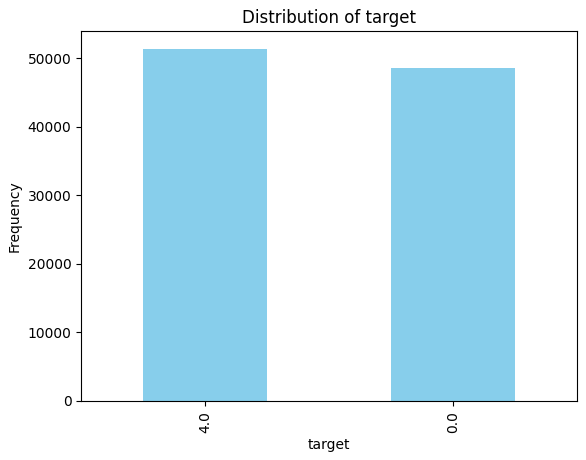
\includegraphics[width=\textwidth]{img/visualize_pic/distribution.png}
%     \caption{The Distribution of Target}
% \end{figure}

\subsection{Relationships of the Attributes}

Complementing this, the \textbf{Pairwise Relationships} Pairplot highlights numerical features such as 'target', 'text\_length', and 'text\_clean\_length'. Histograms show that tweets are generally short, with 'text\_length' peaking at 0–100 characters and 'text\_clean\_length' at 0–40 characters, reflecting the impact of cleaning. Scatter plots reveal no strong correlation between text length and sentiment, while a linear relationship between 'text\_length' and 'text\_clean\_length' confirms the effectiveness of cleaning. These visualizations offer insights into the dataset’s structure for further modeling.

\begin{figure}[H]
    \centering
    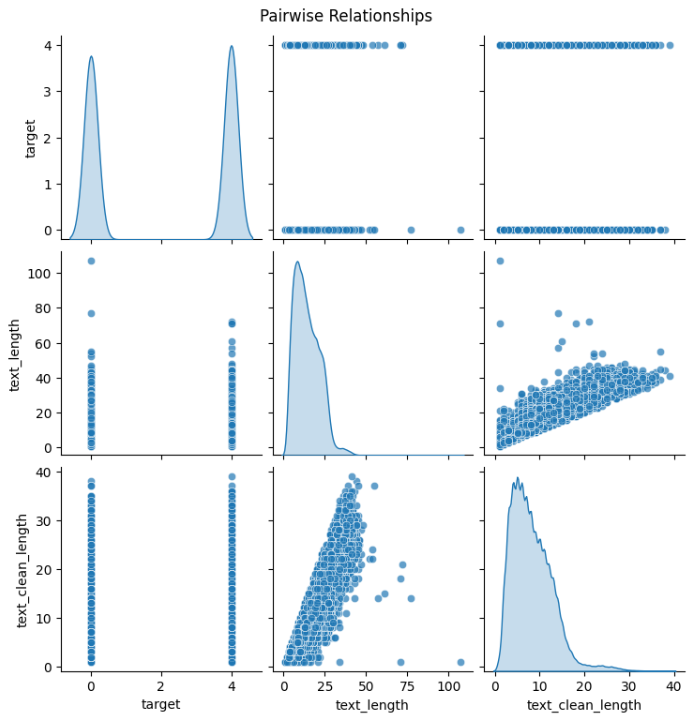
\includegraphics[width=0.8\textwidth]{img/visualize_pic/pairwise.png}
    \caption{Pairwise Relationships}
\end{figure}

\subsection{Top Words Visualizations}

The visualizations highlight the top 20 most frequent words in the 'text\_clean' column through a bar chart and a word cloud. The chart shows 'i' (14,000 occurrences), 'm' (12,000), and 'modi' (10,000) as the most common words, alongside verbs like 'get,' 'like,' and 'go,' and positive terms such as 'good,' 'love,' and 'great.' The word cloud emphasizes high-frequency words like 'i,' 'm,' and 'modi' with larger fonts, while less frequent words like 'great' and 'lol' appear smaller. Together, these visualizations reveal the dataset's informal Twitter tone and frequent sentiment-related terms, offering insights into its linguistic patterns.

\begin{figure}[H]
    \centering
    \begin{subfigure}[b]{0.48\textwidth}
        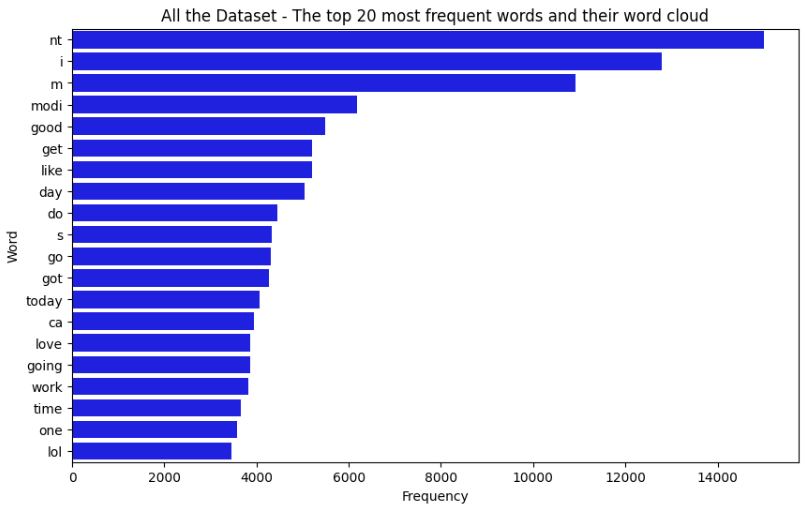
\includegraphics[width=\textwidth]{img/visualize_pic/top20.png}
    \end{subfigure}
    \begin{subfigure}[b]{0.48\textwidth}
        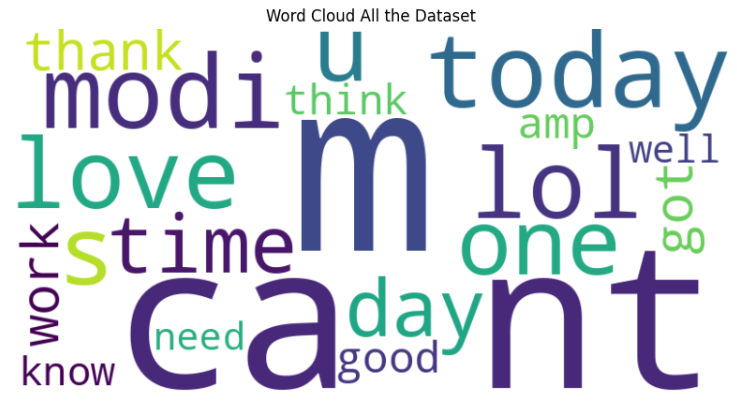
\includegraphics[width=\textwidth]{img/visualize_pic/top20_word_cloud.png}
    \end{subfigure}
    \caption{Top 20 of entire dataset}
\end{figure}

The positive class visualization (target = 4.0) uses a bar chart and word cloud to display the top 20 most frequent words. The bar chart highlights 'i' (5,000 occurrences), 'm' (4,500), and 'modi' (4,000) as the most frequent, followed by positive words like 'good' (3,500), 'love' (3,000), 'thanks' (1,800), and casual terms like 'lol' and 'haha.' The word cloud reinforces this, with larger fonts for frequent words like 'i,' 'm,' and 'good,' and smaller fonts for less common ones like 'haha.' These visualizations emphasize optimism, gratitude, and humor in positive tweets.

\begin{figure}[H]
    \centering
    \begin{subfigure}[b]{0.48\textwidth}
        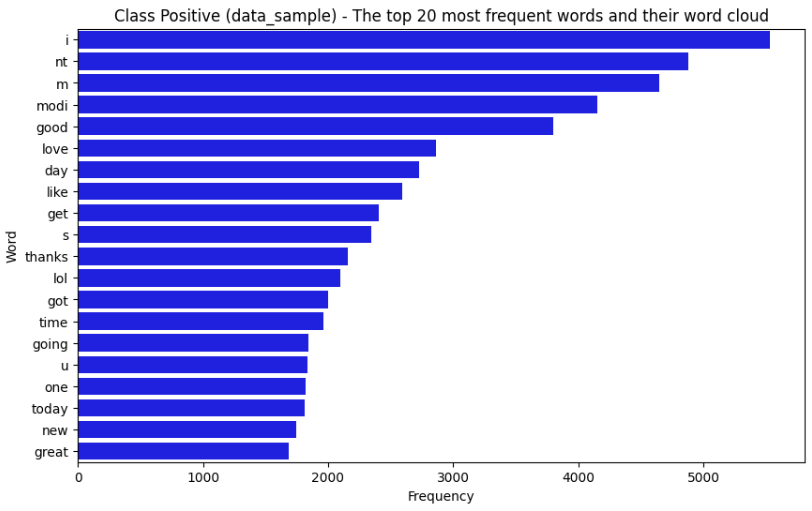
\includegraphics[width=\textwidth]{img/visualize_pic/top20_posi.png}
    \end{subfigure}
    \begin{subfigure}[b]{0.48\textwidth}
        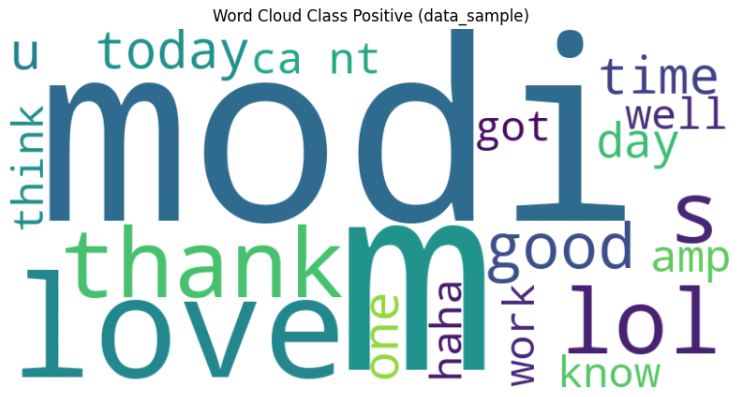
\includegraphics[width=\textwidth]{img/visualize_pic/posi_wordcloud.png}
    \end{subfigure}
    \caption{Top 20 of class Positive}
\end{figure}

The negative class visualization (target = 0.0) uses a bar chart and word cloud to display the top 20 most frequent words. The bar chart shows 'i' (10,000 occurrences), 'm' (9,000), and 'don’t' (8,000) as the most frequent, followed by words like 'get' (7,000), 'go' (6,000), and negative terms such as 'really,' 'want,' 'still,' and 'miss.' The word cloud reinforces this with larger fonts for frequent words like 'i,' 'm,' and 'don’t,' and smaller fonts for less common ones like 'miss.' These visualizations highlight frustration, restriction, and dissatisfaction in negative tweets.

\begin{figure}[H]
    \centering
    \begin{subfigure}[b]{0.48\textwidth}
        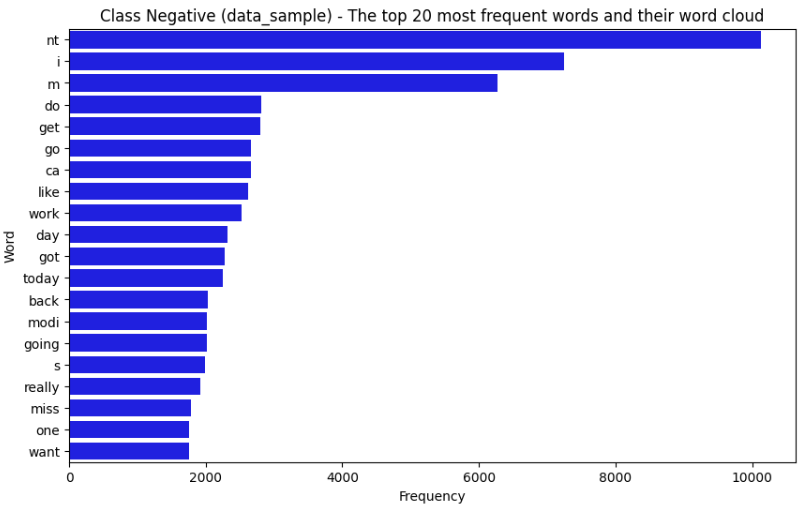
\includegraphics[width=\textwidth]{img/visualize_pic/top20_nega.png}
    \end{subfigure}
    \begin{subfigure}[b]{0.48\textwidth}
        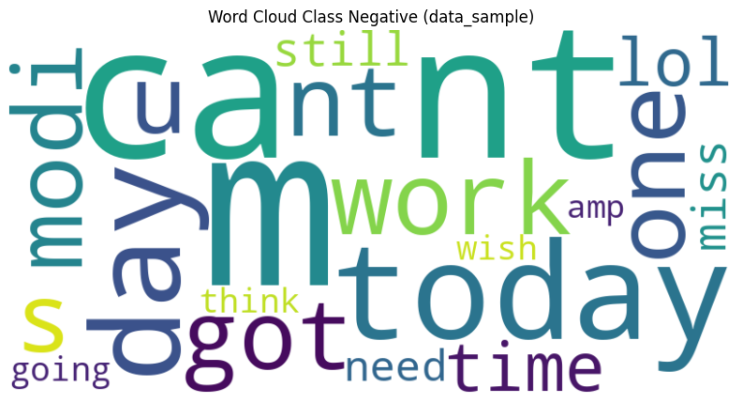
\includegraphics[width=\textwidth]{img/visualize_pic/nega_wordcloud.png}
    \end{subfigure}
    \caption{Top 20 of class Negative}
\end{figure}

\subsection{The distribution of Text Length}

The graphical representations of cleaned tweet lengths (text\_clean\_length) across sentiment classes in the dataset are depicted through a boxplot and histogram. The boxplot indicates that tweets labeled as negative (target = 0.0, in blue) and positive (target = 4.0, in orange) have comparable median lengths, around 10–15 characters, with interquartile ranges extending approximately 5–20 characters. The tighter range (0–40 characters) compared to original text lengths emphasizes the cleaning process’s effect in eliminating unnecessary characters like punctuation and hashtags. Outliers stretching to 35–40 characters are rare and not associated with any particular sentiment, implying that cleaned text length is largely independent of sentiment classification. The histogram complements this by showing that both negative and positive tweets predominantly range between 0 and 10 characters, peaking at about 9,000 for negative tweets and slightly fewer for positive tweets in that range, with frequencies dropping steeply beyond 10 characters and very few tweets surpassing 20 characters. This right-skewed distribution underscores the concise nature of cleaned Twitter data, revealing no significant differences in length distribution between negative and positive sentiments, suggesting that cleaned text length does not play a major role in determining sentiment.

\begin{figure}[H]
    \centering
    \begin{subfigure}[b]{0.48\textwidth}
        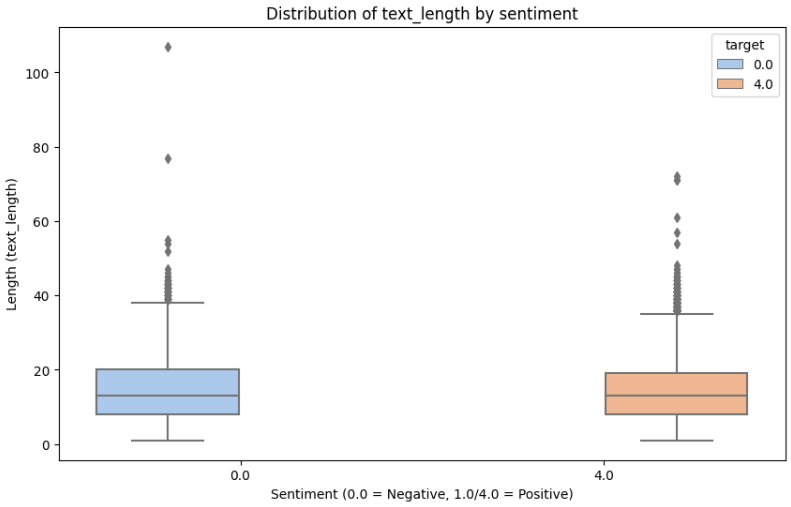
\includegraphics[width=\textwidth]{img/visualize_pic/text_length.png}
    \caption{Distribution of text\_length by sentiment}
    \end{subfigure}
    \begin{subfigure}[b]{0.48\textwidth}
         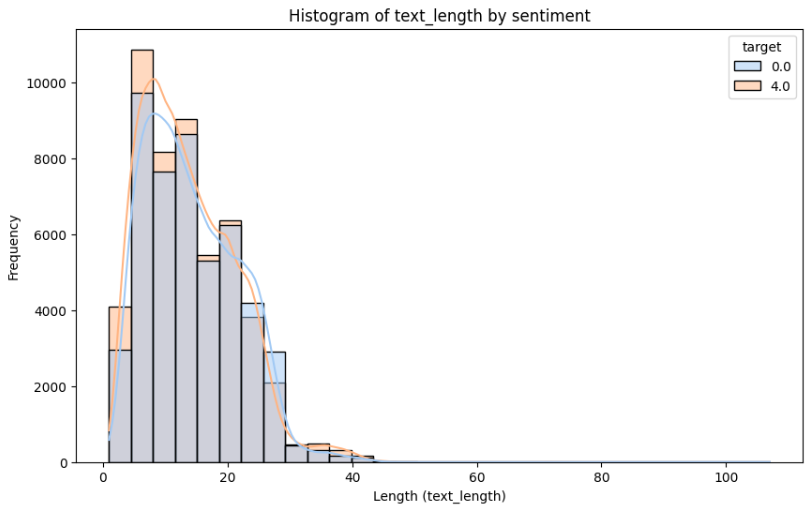
\includegraphics[width=\textwidth]{img/visualize_pic/histogram_text_length.png}
    \caption{Histogram of text\_length by sentiment}
    \end{subfigure}
\end{figure}

The visualizations of cleaned tweet lengths (text\_clean\_length) across sentiment classes in the dataset are illustrated through a boxplot and histogram. The boxplot shows that tweets labeled as negative (target = 0.0, in blue) and positive (target = 4.0, in orange) share similar median lengths, around 10–15 characters, with interquartile ranges spanning roughly 5–20 characters. The narrower range (0–40 characters) compared to original text lengths underscores the cleaning process’s role in removing extraneous characters such as punctuation and hashtags. Outliers reaching up to 35–40 characters are infrequent and not tied to any specific sentiment, indicating that cleaned text length is generally unrelated to sentiment classification. The histogram complements this by revealing that both negative and positive tweets mostly fall between 0 and 10 characters in length, peaking at approximately 9,000 for negative tweets and slightly less for positive tweets in that range, with frequencies declining sharply beyond 10 characters and very few tweets exceeding 20 characters. This right-skewed pattern highlights the concise nature of cleaned Twitter data, showing no notable variation in length distribution between negative and positive sentiments, suggesting that cleaned text length does not significantly affect sentiment determination.

\begin{figure}[H]
    \centering
    \begin{subfigure}[b]{0.48\textwidth}
        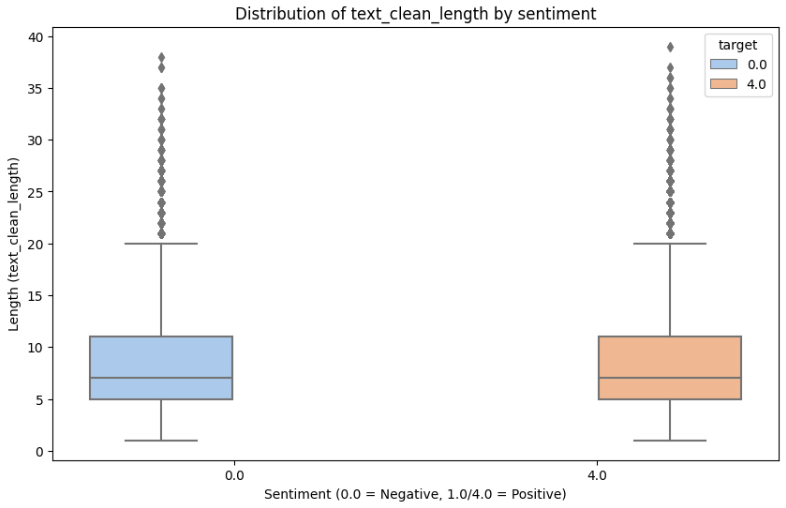
\includegraphics[width=\textwidth]{img/visualize_pic/text_clean.png}
    \caption{Distribution of text\_clean\_length by sentiment}
    \end{subfigure}
    \begin{subfigure}[b]{0.48\textwidth}
         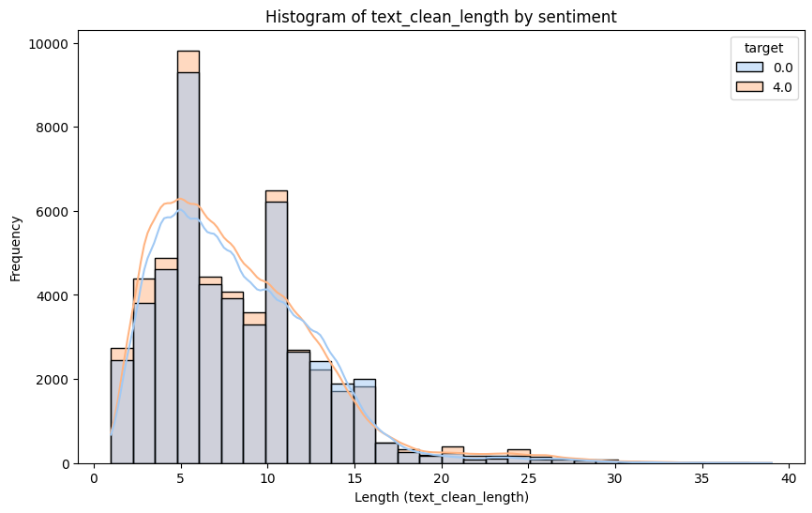
\includegraphics[width=\textwidth]{img/visualize_pic/text_clean_histogram.png}
    \caption{Histogram of text\_clean\_length by sentiment}
    \end{subfigure}
\end{figure}

\subsection{Word Frequencies by Labels}

A heatmap delivers a comprehensive analysis of word frequencies by sentiment, enabling trends to be identified quickly at a glance. It displays the same words—“day,” “going,” “good,” “got,” “like,” “lol,” “love,” “m,” “modi,” “nt,” “s,” “thanks,” “today,” and “work”—with color intensity indicating frequency, ranging from light yellow (representing low frequency, such as 0 occurrences) to dark red (indicating high frequency, for example, 10,130 for “modi” in negative tweets). For instance, “modi” emerges as a prominent term in negative tweets, marked by a deep red shade, while “good” and “love” shine vividly in positive tweets, underscoring their connection to positivity. Together, these representations create a clear and dynamic portrayal of the dataset’s linguistic patterns, emphasizing how word usage mirrors underlying sentiments and providing valuable insights for deeper analysis.

\begin{figure}[H]
    \centering
    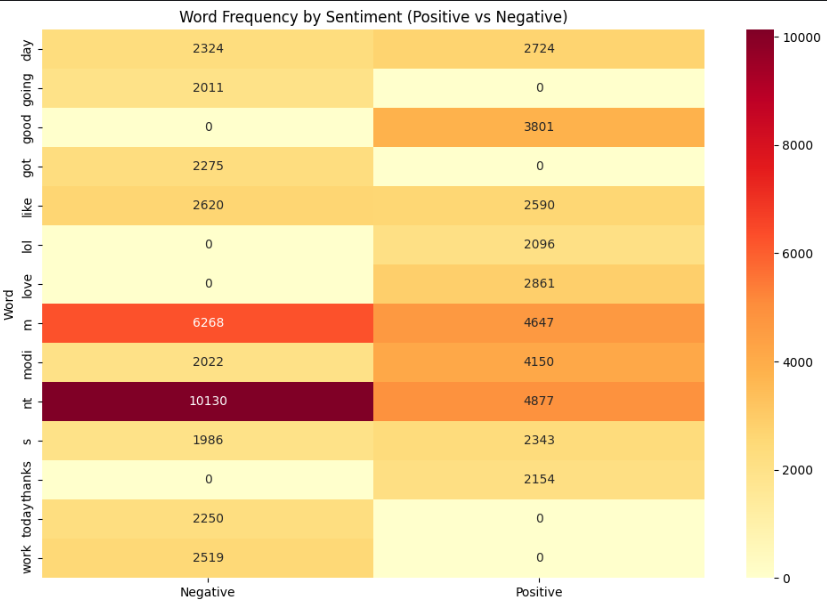
\includegraphics[width=\textwidth]{img/visualize_pic/word_frequency.png}
    \caption{Word Frequency by Sentiment}
\end{figure}

A bar chart provides a straightforward comparison of word frequencies across positive and negative sentiments, illustrating how specific words differ in usage. It shows that terms like “modi” and “m” appear much more frequently in negative tweets, with “modi” recorded around 10,130 times and “m” at 6,268 times, in contrast to 4,877 and 4,647 times in positive tweets, respectively. On the other hand, positive tweets exhibit greater occurrences of words such as “good” (3,801 times) and “love” (2,861 times), which are largely absent or scarce in negative tweets. This striking contrast highlights the unique emotional undertones, with negative tweets often reflecting frustration or limitation, while positive tweets express optimism and warmth.

\begin{figure}[H]
    \centering
    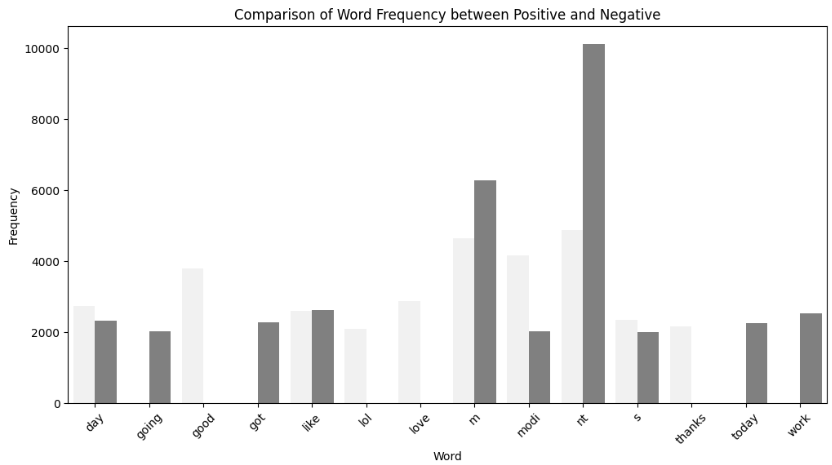
\includegraphics[width=\textwidth]{img/visualize_pic/comparision.png}
    \caption{Comparision of Word Frequency}
\end{figure}

\newpage
